\chapter{Bitcity}

Por ser uma linguagem moderna, Java possui suporte a concorrência e a
tratamentos de exceções, como visto no Capítulo \ref{cha:concjava}. Agora 
será visto como esses recursos foram empregados no desenvolvimento da
\textbf{Bitcity}.

A \textbf{Bitcity} parte de um modelo textual para projetar um mundo
onde retângulos azuis representam carros que respeitam os semáforos
mas que não apreciam congestionamento, esporadicamente
retângulos brancos surgem e representam uma ambulância que age como um
coletor de recursos, folhas crescem em árvores e a chuva faz as mesmas
caírem.

O Modelo \ref{short-one} apresenta todos os elementos que podem ser
encontrados no modelo textual.

\begin{model}
\centering
\begin{BVerbatim}
9 18 3 2 15
######           #
*>  -#           #
$..$-#           # 
$..$A#############
*> A-     B>>
###$ ######B #####
  #$ #    #  #    
  #$> &   #+ #####
###$ #    #+    <*
\end{BVerbatim}
  \caption{Exemplo demonstrativo \label{short-one}}
\end{model}

A primeira linha contém quatro inteiros que descrevem, respectivamente,
quantidade de linhas, quantidade de colunas, número de pontos de
partida, número de conjuntos de semáforos a serem sincronizados e a
quantidade máxima de carros no mundo num dado instante.

O caractere \verb!`#'! representa calçada, \verb!`&'! é um
estacionamento, \verb!`$'! representa
vegetação rasteira, \verb!`.'! uma árvore que ganha e perde folhas ao
longo da execução, uma letra qualquer que se repete indica semáforos
que pertencem a um mesmo conjunto. Os pontos de partida, que ficam
responsáveis por indicar os locais onde carros surgem no mundo, são
representados por \verb!`*'!. Os símbolos \verb!`+'!, \verb!`-'!,
\verb!`>'! e \verb!`<'! indicam, respectivamente, para cima, para
baixo, esquerda e direita e são utilizados pelos veículos para
movimentação no mundo.

O modelo é projetado de forma a simplificar a construção do mundo e
também o \textit{parsing} do mesmo. Todo ponto de partida precisa,
necessariamente, que uma direção inicial esteja presente ou
imediatamente a sua direita, ou a esquerda, ou em cima ou
embaixo. Essa direção define a direção de deslocamento inicial de
todos os carros que partirem daquele ponto. Os carros possuem uma
unidade de visão à sua frente, considerando sua direção atual. Esta
visão é utilizada para tomada de seis decisões:
\begin{description}
\item[Mudar direção atual]: O elemento à frente contém um dos
  caracteres que indicam uma direção e à frente deste outro caractere,
  considerando a direção que representa, o símbolo se repete. Esse
  caso ocorre no Modelo \ref{short-one} na linha 2, coluna 5.
\item[Escolher entre mudar de direção ou não]: O elemento à frente
  contém um dos caracteres que indicam uma direção e à frente deste
  outro caractere, considerando a direção que representa, o símbolo
  não se repete. Situação da linha 5, coluna 5 no Modelo
  \ref{short-one} e também na linha 8, coluna 5 para entrar em uma garagem.
\item[Parar no semáforo]: Veículo, exceto ambulância, depara-se com
  sinal vermelho e obrigatoriamente para.
\item[Buzinar]: O sinal está aberto, porém existe um veículo a sua
  frente que está parado.
\item[Sair do mundo]: O veículo atingiu o limite do mundo ou um
  estacionamento. No Modelo
  \ref{short-one} essa situação pode ocorrer ao atingir tanto uma
  linha após a 9 na coluna 5, uma coluna após a 18 na linha 5 ou
  a linha 8, coluna 7.
\item[Deslocar-se]: Posição à frente não contém nenhum elemento
  especial, o veículo pode continuar deslocando-se seguindo sua
  direção corrente.
\end{description}
Além disso, todos os pontos de partida devem estar ligados -- no mesmo
sentido de um grafo conexo. Deve ser possível atingir todos os outros
pontos partindo de qualquer um deles, sem considerar a direção de
deslocamento de veículos.

A aplicação espera iniciar sua execução com um modelo que se adeque as
especificações a cima. Caso isso não ocorra, a classe \verb!Parser!
fica responsável por detectar o problema e levantar uma exceção. A
classe \verb!Application! fica responsável por tratar esta exceção,
sendo exibido o erro encontrado e abortando a execução da aplicação.
Recebendo um modelo correto, a aplicação trata de renderizar o mundo
especificado. A classe \verb!WorldMap! que estende a classe
\verb!JPanel! e implementa a interface \verb!Runnable! fica
responsável por essa tarefa. Na implementação atual, essa renderização
é bastante simplificada, sendo feito uso de recursos simples como
retângulos e círculos que são desenhados através de métodos existentes
da classe \verb!Graphics2D!. As Figuras \ref{fig1} e \ref{fig2} exibem
o resultado desta etapa para o Modelo \ref{short-one} em momentos
distintos durante a execução.

\begin{figure}[ht!]
  \centering
  \subfigure[Árvores crescendo, deslocamento de carros, outros detalhes \label{fig1}]{
    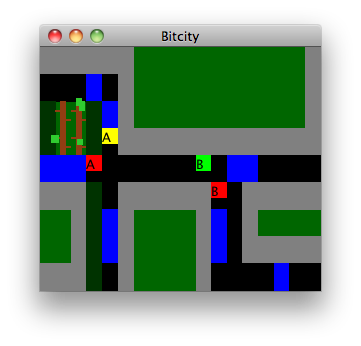
\includegraphics[scale=0.58]{figs/map1_1.png}
  }
  \subfigure[Chovendo no mundo, carro com retângulo branco buzinando \label{fig2}]{
    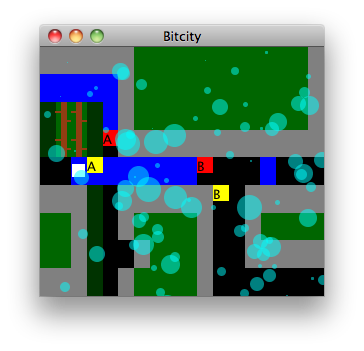
\includegraphics[scale=0.58]{figs/map1_2.png}
  }
  \caption{Modelo \ref{short-one} renderizado}
\end{figure}

A distinção entre ruas e vegetação comum exibida não requer elementos
especiais no modelo textual. O algoritmo \textit{4-way flood fill} é
aplicado a um ponto de partida qualquer e todas as posições atingidas,
considerando que calçada, garagem e vegetação rasteira são bordas
nesse preenchimento, são coloridas de preto. Isso colore todas as ruas
devido a restrição dos pontos serem ligados. Em relação a calçadas e
estacionamentos, atualmente não há distinção visual entre os dois
elementos.

A renderização do mundo ocorre em um \textit{thread} a parte, sendo
esta criada durante a inicialização da aplicação. É permitido ajustar
a velocidade da taxa de atualização, ou \textit{Frames Per Second} (FPS),
durante a execução, podendo variar de 30 a 45 renderizações por
segundo do mundo por completo. Durante estas atualizações também
decide-se entre criar um novo carro (classe \verb!Car!) ou não,
inserir uma ambulância ou não, iniciar chuva e também brotar folhas em
árvores.

Além da \textit{thread} principal e da \textit{thread} para desenho,
cada instância de classes que tem como pai a \verb!WorldObject! também
é uma \textit{thread}. Isso inclui todos os veículos que vão sendo
criados, todas as árvores, os sinais de trânsito e chuva.

A sincronização entre semáforos de um mesmo grupo deve ser realizada
para garantir que apenas um deles permaneça aberto durante um período
de tempo, eliminando a ocorrência de acidentes neste mundo ideal. Para
cada letra encontrada no modelo, uma instância da classe
\verb!TrafficLight! é criada e cada um destes recebe uma instância da
classe \verb!Semaphore! que controla os estados de um sinal de
trânsito. Isso é realizado de forma que um mesmo conjunto de letras
receba a mesma instância de um \verb!Semaphore! e, juntamente com a
\textit{keyword} \verb!synchronized! da linguagem Java, assim,
consegue-se limitar o acesso ao método \verb!Semaphore.open! a uma
única instância de um dado conjunto de \verb!TrafficLight!.

Também é feito uso do recurso de sincronização fornecido pela
\verb!synchronized! para avisar (ou alertar) a instância da classe
\verb!Rain! quando deve-se iniciar a chuva. Esse controle é feito da
seguinte forma: ao iniciar a \textit{thread} de \verb!Rain!, ela
invoca o método \verb!Thread.wait! com sincronização no objeto da
instância e, durante a execução da aplicação, a \textit{thread} de
\verb!WorldMap! sincroniza com o mesmo objeto mas faz uso do método
\verb!Thread.notify! para comunicar a \textit{thread} de \verb!Rain!
que esta deve começar a fazer chover. A determinação de quando o
método \verb!Thread.notify! é de fato chamado depende do sorteio de
números aleatórios e também da satisfação da condição de já não estar
chovendo.

Um último recurso de destaque no mundo é a ambulância, criada por meio
da classe \verb!Ambulance!. É permitido que somente uma desta esteja
no mundo ao mesmo tempo e ela só é criada caso o total de carros em
circulação seja superior a quantidade $max - 4$. Uma ambulância age
como uma forma de coletor de \textit{threads}, destruindo carros que
estejam em seu caminho e que não se desloquem ao mesmo tempo em que a
ambulância passa. Isso é feito pois a criação de linhas de execução
extras consome espaço no \textit{heap}, sendo possível ultrapassar o
limite disponível com mapas maiores que comportam uma grande
quantidade de carros ao mesmo tempo.% XXX Falar ainda do problema que
%isso vai causar XXX. XXX Colocar alguma referencia em relação ao
%tamanho variável que uma thread pode ocupar em heap quando criada XXX.

A remoção de veículos no mundo ocorre por meio do uso de exceções. No
momento em que um carro toma a decisão de sair do mundo, uma exceção é
levantada e o método \verb!run! do respectivo objetivo trata essa
situação como encerramento da \textit{thread}. No caso de ambulância
também é feito uso da \textit{keyword} \verb!finally! para garantir
que um efeito sonoro, que é iniciado ao instanciar uma ambulância,
seja desativado. Em outros momentos onde ocorre a utilização de
efeitos sonoros, também é feito uso de tratamento de exceções para
garantir que problemas de: falta de suporte ao formato de audio,
arquivo inexistente ou dispositivo de som ocupado; não causem um
encerramento prematura da aplicação.

\section{Hierarquia de Classes}

A Figura \ref{hierarchy} apresenta a hierarquia das classes da
\textbf{Bitcity}.

\begin{figure}[ht!]
  \centering
  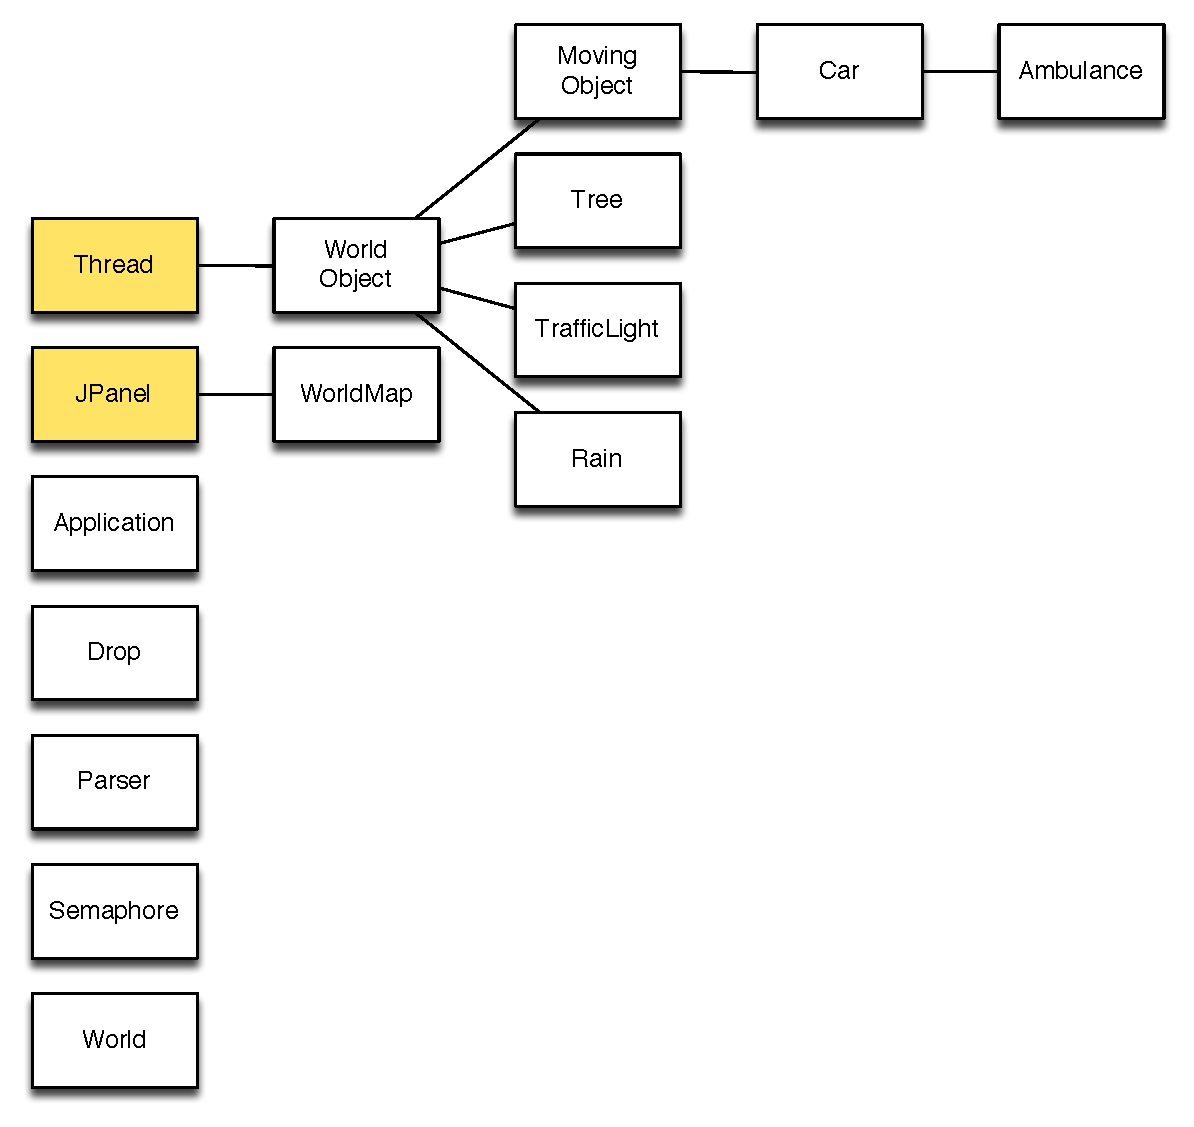
\includegraphics[scale=0.58]{figs/hierarchy}
  \caption{Classes em amarelo percentem a Java, em branco a aplicação \label{hierarchy}}
\end{figure}

A classe \verb!Application! ficou responsável por implementar o método
\verb!main! e iniciar a execução da aplicação. A classe \verb!Drop! é
utilizada pela \verb!Rain! para desenhar as gotas de chuva. Por
último, a \verb!TrafficLight! faz uso da \verb!Semaphore! para
controlar o tráfego.
